\documentclass[12pt, twoside]{article}
\usepackage[letterpaper, margin=1in, headsep=0.5in]{geometry}
\usepackage[english]{babel}
\usepackage[utf8]{inputenc}
\usepackage{amsmath}
\usepackage{amsfonts}
\usepackage{amssymb}
\usepackage{tikz}
\usepackage{yhmath}
\usetikzlibrary{quotes, angles}
\usepackage{graphicx}
\usepackage{enumitem}
\usepackage{multicol}

\newif\ifmeta
\metatrue %print standards and topics tags

\title{Regents Geometry}
\author{Chris Huson}
\date{April 2022}

\usepackage{fancyhdr}
\pagestyle{fancy}
\fancyhf{}
\renewcommand{\headrulewidth}{0pt} % disable the underline of the header
\raggedbottom

\fancyhead[LE]{\thepage}
\fancyhead[RO]{\thepage \\ Name: \hspace{4cm} \,\\}
\fancyhead[LO]{BECA / Dr. Huson / Geometry\\* Mixed Review\\* 2 May 2022}

\begin{document}
\subsubsection*{11.1 Quiz Trigonometry \hfill HSG.SRT.C.8}
\begin{enumerate}
\item Points that are all located on the same plane are $\rule{4cm}{0.15mm}$.\bigskip

\item Identify three points in the given plane.\\[0.25in]
  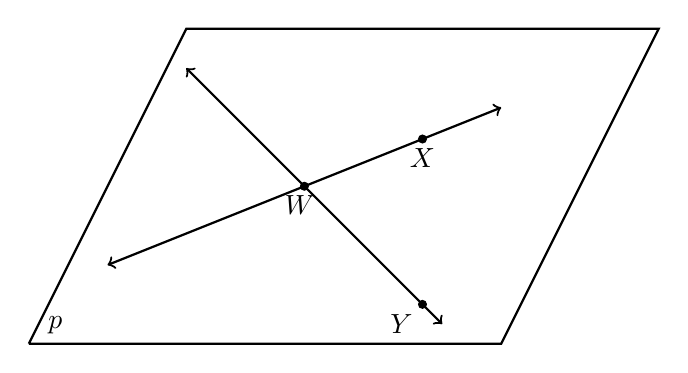
\begin{tikzpicture}
    \draw [thick](0,0) node[above right]{$\ p$} --(6,0)--(8,4)--(2,4)--(0,0);
    \draw [<->, thick] (1,1)--(6,3);
    \draw [fill] (3.5,2) circle [radius=0.05] node[below]{$W \ $};
    \draw [fill] (5,2.6) circle [radius=0.05] node[below]{$X$};
    \draw [<->, thick] (2,3.5)--(5.25,.25);
    \draw [fill] (5,0.5) circle [radius=0.05] node[below left]{$Y$};
  \end{tikzpicture} \vspace{1cm}

\item Given $\overline{ABC}$, $AB=3x-4$, $BC=x+5$, $AC=13$. Find ${BC}$. \\ 
  Check your answer for full credit.
  \vspace{1cm}
    \begin{center}
      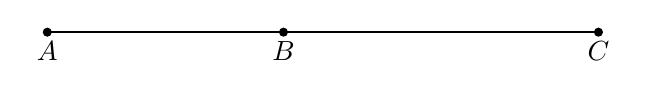
\begin{tikzpicture}
          \draw [-, thick] (0,0)--(7,0);
          \draw [fill] (0,0) circle [radius=0.05] node[below]{$A$};
          \draw [fill] (3,0) circle [radius=0.05] node[below]{$B$};
          \draw [fill] (7,0) circle [radius=0.05] node[below]{$C$};
      \end{tikzpicture}
    \end{center}

\item Given $\overleftrightarrow{PQ}$ as shown on the number line, with $P=-3$ and $Q=5.5$. \\[20pt] % Midpoint
  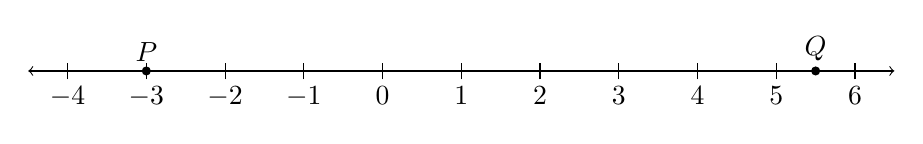
\begin{tikzpicture}
    \draw [<->] (-4.5,0)--(6.5,0);
    \foreach \x in {-4,...,6} %2 leading for diff!=1
      \draw[shift={(\x,0)},color=black] (0pt,-3pt) -- (0pt,3pt) node[below=5pt]  {$\x$};
      \draw [fill] (-3,0) circle [radius=0.05] node[above] {$P$};
      \draw [fill] (5.5,0) circle [radius=0.05] node[above] {$Q$};
  \end{tikzpicture} \\ \bigskip
  What is the exact distance on the number line between the points $P$ and $Q$?

\item Given $\overline{WXYZ}$, $WX=3 \frac{1}{2}$, $XY=4 \frac{3}{4}$, and $YZ= 1 \frac{1}{4}$. \\ [0.25cm]
Find ${WZ}$.\\[.5in]
  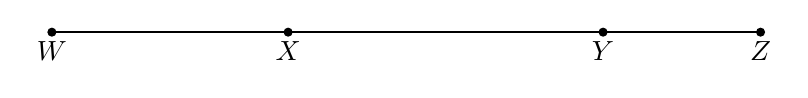
\begin{tikzpicture}
    \draw [-, thick] (0,0)--(9,0);
    \draw [fill] (0,0) circle [radius=0.05] node[below]{$W$};
    \draw [fill] (3,0) circle [radius=0.05] node[below]{$X$};
    \draw [fill] (7,0) circle [radius=0.05] node[below]{$Y$};
    \draw [fill] (9,0) circle [radius=0.05] node[below]{$Z$};
  \end{tikzpicture}
  
\item Given the points $V$ and $W$, draw $\overrightarrow{WV}$.\\
\vspace{1cm}
\begin{center}
  \begin{tikzpicture}
  \draw [fill] (0,2) circle [radius=0.05] node[below]{$V$};
  \draw [fill] (5,0) circle [radius=0.05] node[below]{$W$};
\end{tikzpicture}
\end{center}

\item Use symbols to write the name of each geometric figure.\\.\\
  \vspace{0.5cm}
  \begin{tikzpicture}
    \draw [->, thick] (0,0)--(3,1.5);
    \draw [fill] (0,0) circle [radius=0.05] node[below]{$G$};
    \draw [fill] (2,1) circle [radius=0.05] node[below]{$H$};
    \node at (-1,0) {(a)};
  \end{tikzpicture}  \hspace{.1cm}
  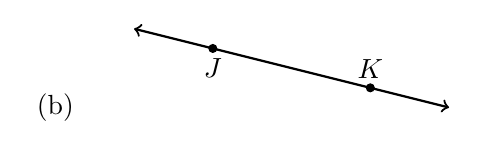
\begin{tikzpicture}
    \draw [<->, thick] (1,1)--(5,0);
    \draw [fill] (2,0.75) circle [radius=0.05] node[below]{$J$};
    \draw [fill] (4,.25) circle [radius=0.05] node[above]{$K$};
    \node at (0,0) {(b)};
  \end{tikzpicture} \hspace{.25cm}
  \begin{tikzpicture}
    \draw [-, thick] (1,0)--(4,2);
    \draw [fill] (1,0) circle [radius=0.05] node[below]{$L$};
    \draw [fill] (4,2) circle [radius=0.05] node[above left]{$M$};
    \node at (0,0) {(c)};
  \end{tikzpicture}

\item Given $\triangle ABC$ with $\overline{AB} \cong \overline{AC}$. On the diagram mark the congruent line segments with tick marks.
\begin{center}
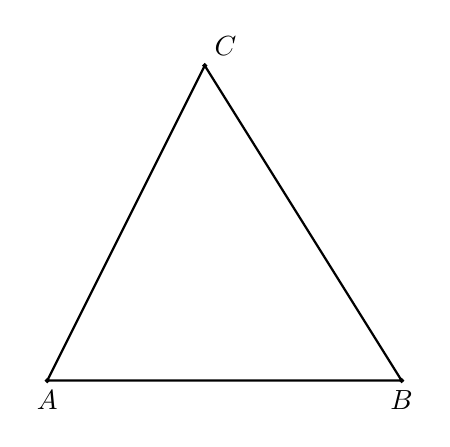
\begin{tikzpicture}[scale=0.5]
  \draw [thick](0,0)--(9,0)--(4,8)--(0,0);
  \draw [fill] (0,0) circle [radius=0.05] node[below]{$A$};
  \draw [fill] (9,0) circle [radius=0.05] node[below]{$B$};
  \draw [fill] (4,8) circle [radius=0.05] node[above right]{$C$};
\end{tikzpicture}
\end{center}

\item Find the measure of the angle in degrees and the given segment's length in centimeters. \vspace{0.25cm}
\begin{enumerate}
  \item  $m \angle GEF = $ \rule{4cm}{0.15mm} \bigskip
  \item  $EG=$ \rule{4cm}{0.15mm} \bigskip
  \item Name a pair of opposite rays: \rule{4cm}{0.15mm} \bigskip
\end{enumerate}
\begin{center}
\begin{tikzpicture}[scale=1.5]
  \draw [->, thick] (0,0)--(35:5);
  \draw [<->, thick] (-3,0)--(7,0);
  %\draw [->, thick] (0,0)--(-1.2,3);
  %\draw [fill] (-1,2.5) circle [radius=0.05] node[left ]{$B$};
  \draw [fill] (35:3) circle [radius=0.05] node[above left ]{$G$};
  \draw [fill] (-2,0) circle [radius=0.05] node[below]{$D$};
  \draw [fill] (0,0) circle [radius=0.05] node[below]{$E$};
  \draw [fill] (4,0) circle [radius=0.05] node[above]{$F$};
\end{tikzpicture}
\end{center}

\item Use each term according to its geometric meaning: ``sketch", ``draw", ``construct".
\begin{enumerate}
  \item $\rule{4cm}{0.15mm}$ is to make a freehand diagram showing important features. \smallskip
  \item $\rule{4cm}{0.15mm}$ is to depict with accurate measures using ruler, protractor, and compass. \smallskip
  \item $\rule{4cm}{0.15mm}$ is a formal, logical process to create geometric figures using only a straightedge and compass.
\end{enumerate} \smallskip

\item Given the situation in the diagram, answer each question. Circle True or False. \vspace{0.25cm}
    \begin{flushright}
    \begin{tikzpicture}[scale=1]
      \draw [->, thick] (0,0)--(50:5);
      \draw [<->, thick] (-5,.5)--(5,-.5);
      \draw [->, thick] (0,0)--(-1.2,3);
      \draw [fill] (-1,2.5) circle [radius=0.05] node[left ]{$S$};
      \draw [fill] (50:3) circle [radius=0.05] node[above left ]{$T$};
      \draw [fill] (0,0) circle [radius=0.05] node[below]{$P$};
      \draw [fill] (4,-0.4) circle [radius=0.05] node[above]{$U$};
      \draw [fill] (-4,0.4) circle [radius=0.05] node[above]{$R$};
    \end{tikzpicture}
    \end{flushright}
  \begin{enumerate}
    \item True or False: $\overrightarrow{PR}$ and $\overrightarrow{PU}$ are opposite rays.\bigskip
    \item True or False: $\angle TPR$ is an obtuse angle.\bigskip
    \item True or False: $\angle RPS$ and $\angle TPU$ are adjacent angles. \bigskip
  \end{enumerate}

\item Given the rectangle $ABCD$ shown below, with $AB=12$ and $BC=5$. The diagonal $\overline{AC}$ is drawn to create two triangles. Find the area of the lower triangle, $\triangle ABC$.
\begin{flushleft}
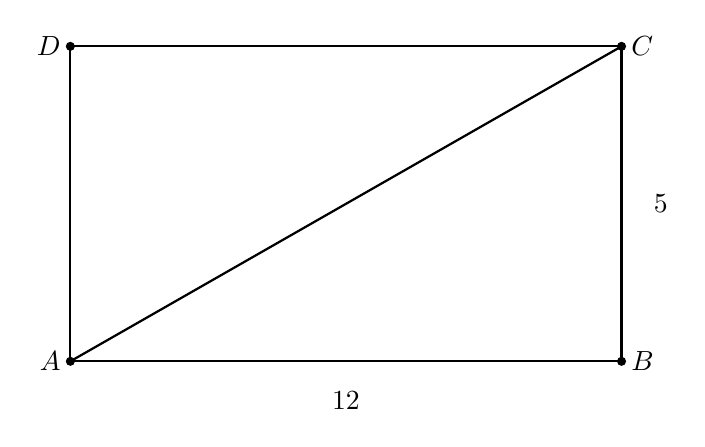
\begin{tikzpicture}
  \draw [-, thick] (0,0)--(7,0)--(7,4)--(0,4)--cycle;
  \draw [-, thick] (0,0)--(7,4);
  \draw [fill] (0,0) circle [radius=0.05] node[left]{$A$};
  \draw [fill] (7,0) circle [radius=0.05] node[right]{$B$};
  \draw [fill] (7,4) circle [radius=0.05] node[right]{$C$};
  \draw [fill] (0,4) circle [radius=0.05] node[left]{$D$};
  \node at (7.5, 2){5};
  \node at (3.5, -0.5){12};
\end{tikzpicture}
\end{flushleft}

\item A student constructs a triangle with a given side, $\overline{AB}$ as shown below. Is $\triangle ABC$ equilateral? Justify your answer by explaining what was done incorrectly and how it should have been done.
  \begin{flushleft}
  \begin{tikzpicture}[scale=0.7, rotate=-20]
    \draw [-, thick] (0,0)--(5,0)--(66.4:4)--cycle;
    \draw [fill] (0,0) circle [radius=0.05] node[left]{$A$};
    \draw [fill] (5,0) circle [radius=0.05] node[right]{$B$};
    \draw [fill] (66.4:4) circle [radius=0.05] node[above]{$C$};
    \draw (0,0) circle [radius=4];
    \draw (5,0) circle [radius=5];
  \end{tikzpicture}
  \end{flushleft}

\newpage
\item In the following two problems, solve for the value of $x$.
\begin{multicols}{2}
  \begin{enumerate}
    \item   $3(x-5)=-33$ \vspace{6cm}
    \item   $3-\frac{1}{2} x=2$ \vspace{6cm}
  \end{enumerate}
\end{multicols}

\item In the following two problems, solve for the value of $x$ by factoring.
  \begin{multicols}{2}
    \begin{enumerate}
      \item   $x^2+6x=-5$ \vspace{6cm}
      \item   $x^2=x+12$ \vspace{6cm}
    \end{enumerate}
  \end{multicols}

\end{enumerate}
\end{document}
  